% Please use the skeleton file you have received in the 
% invitation-to-submit email, where your data are already
% filled in. Otherwise please make sure you insert your 
% data according to the instructions in PoSauthmanual.pdf
\documentclass{PoS}

\title{The $\gamma$-ray Milky Way above 10 GeV:\\
Distinguishing Sources from Diffuse Emission}

\ShortTitle{Distinguishing Sources from Diffuse Emission}

\author{\speaker{E. Owen},$^a$ C. Deil,$^{a}$ A. Donath,$^{a}$ R. Terrier$^{b}$\\
\llap{$^a$}Max-Planck-Institut f\"{u}r Kernphysik, P.O. Box 103980, D
69029 Heidelberg, Germany\\
\llap{$^b$}Astroparticule \& Cosmologie, CNRS, 75205 Paris Cedex 13, France\\
E-mail: \email{ellis.owen@mpi-hd.mpg.de}, \email{christoph.deil@mpi-hd.mpg.de}, \email{axel.donath@mpi-hd.mpg.de}, \email{terrier@apc.univ-paris7.fr}}


\abstract{One of the most prominent features of the gamma-ray sky is the emission from our own galaxy. The Galactic plane has been observed by \textit{Fermi}/LAT in GeV and H.E.S.S. in TeV light. Fermi has modeled the Galactic emission as the sum of a complex "diffuse" emission model with the predominately point source catalogs of 1FHL and 2FGL, while H.E.S.S. has primarily detected extended TeV sources. At GeV energies, Galactic diffuse emission dominates the gamma-ray Milky Way but, as sources have hard spectra, it is likely their emission dominates at TeV energies. Generally the spatial shape and fraction of source emission compared to diffuse emission in the Galactic plane is not well known and is dependent on the source detection method, threshold and diffuse emission modeling methods used. \\

We present simple image-analysis based methods applied to Fermi data from 10 GeV to 500 GeV, covering a region of +/- 5 degrees in Galactic latitude and +/- 100 degrees in Galactic longitude, to separate source and diffuse emission. These methods include significance clipping to exclude sources combined with elongated filter smoothing and template fitting with Planck and a Gaussian band model. We compare these methods with one another, and also against models based on the Fermi 1FHL catalog, and apply them to very simple model Galaxies to test the response for an input of known fraction and shape of diffuse and source emission.}

\FullConference{Science with the New Generation of High Energy Gamma-ray experiments, 10th Workshop - Scineghe2014\\
		04-06 June 2014\\
		Lisbon - Portugal}
    
\usepackage{multirow}
\usepackage{gensymb}
\usepackage{wrapfig}
\usepackage{amsmath}
\usepackage{wasysym}
\begin{document}

\section{Introduction}
\subsection{Motivation}
There is a need in the community to find ways of reliably and automatically seperating sources from background emission. This may be for the purpose of better understanding sources for which background contributions are removed, for instance in the development of galactic diffuse models \cite{Fermidiffuse}, construction of source catalogs \cite{1fhl,hgps} or for the improvement of background subtraction methods for source or region morphology studies. 

Alternatively, applications also exist for cases where sources must be removed instead of background, for instance galacitc diffuse emission studies \cite{Egberts} or in the analysis of extended galactic or extragalactic sources [example reference?].

While at lower energies, many methods are be successfully devised to separate source and background emission [example reference??], the challenge lies in finding successful methods for the high-energy GeV and TeV regime where available datasets are increasingly limited by the number of cosmic rays observed.

\subsection{Galactic Emission}
At GeV and TeV energies, galactic emission may be split into three components; sources, truly galactic diffuse emission and the flux contributed by sources as yet to be resolved. While definitions in the literature vary, particularly with regard to unresolved and truly diffuse emission contributions, this study adopts the following convention (as illustrated in Figure 1).
\begin{itemize}
\item{\textbf{Sources} refers to known, observable source above a given instrument detection threshold.}
\item{\textbf{Unresolved sources} are those sources which exist but fall below the detection threshold of a given instrument, and so are not recognised as distinct sources}
\item{\textbf{Truly diffuse galactic emission} refers to the flux contribution from physical processes leading to diffuse cosmic ray emission - at higher TeV energies, this tends to be dominated by inverse Compton and $\pi^0$ decay while at lower GeV energies bremsstrahlung also contributes significantly.}
\item{\textbf{Galactic background emission} refers to the galactic flux contribution which cannot be directly attriubuted to sources. This may be considered as the sum of the unresolved and truly diffuse emission contributions.}
\end{itemize}

In this work, we study methods of separating sources from galactic background emission using image-based techniques at energies above 10 GeV in order to understand appropriate methods for automatic background modelling and source detection.

\begin{figure}[h!]
  \centering
      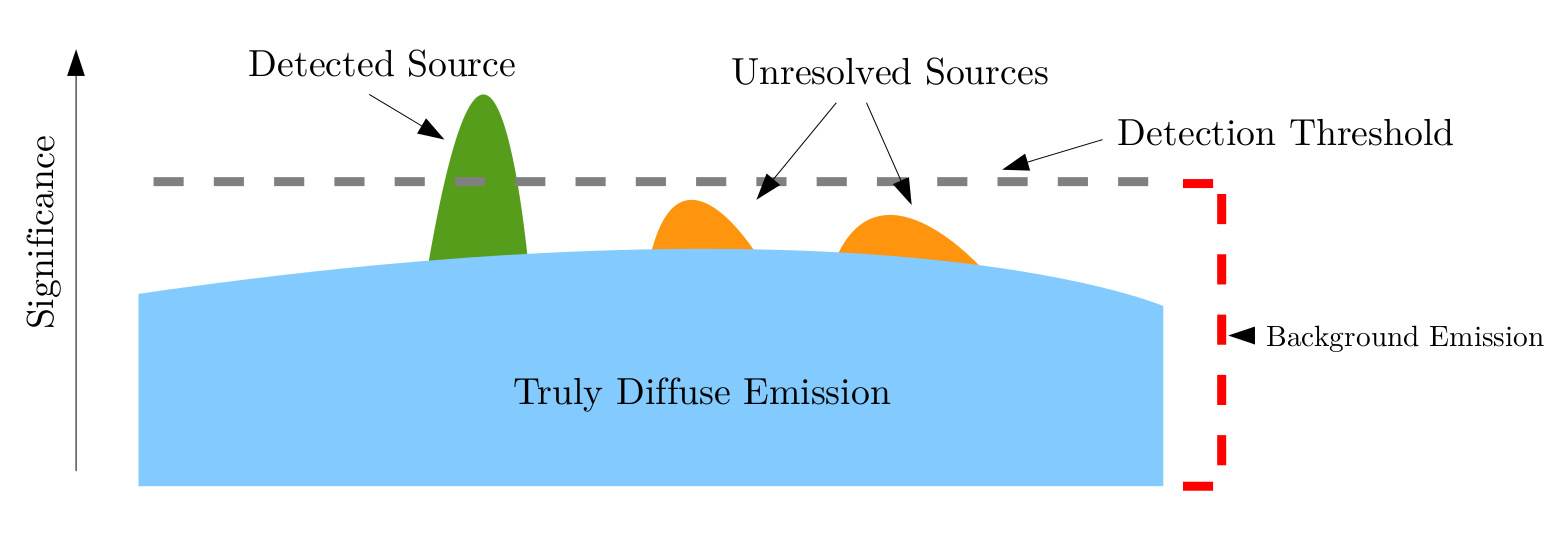
\includegraphics[width=0.75\textwidth]{figures/definitions.png}
  \caption{Illustration for galactic emission definitions.}
\end{figure}

\section{Separation Algorithm}


The initial algorithm that is tested in this study is based on significance clippings. Further methods should be considered in future work. The separation algorithm may be summarised in 4 steps for an input map of detected $\gamma$-ray events, known as a `counts map'.

\begin{itemize}
\item{\textbf{Initiation step:} Counts map is convolved with a background kernel to act as an initial background image.}
\item{\textbf{Propagation step:} A significance image is computed from the counts map and background image. From this, an exclusion mask is determined, removing regions above a set significance threshold, and replacing these regions the respective values from the initial background image. The result is a (new) background image. The step repeats.}
\item{\textbf{Termination step:} Once there is no change in the background image or exclusion mask, the propagation step ends and the final background image is returned.}
\end{itemize}


\subsection{Algorithm Parameters}

A number of parameters must be chosen for this iterative significance-clipping background estimator. Preliminary work and reasoning was used to select initial values for this study, summarised in table 2.

To determine the significance cut-off parameter, a uniform input for the galactic region was taken and poisson flucctuated. The algorithm was then applied for various significance cut-offs, and the final value was chosen when it could be seen that no regions were excluded such that the algorithm didn't identify poisson up-flucctuations as sources. The correlation radius and mask dilation radius were initially chosen here to be roughly equivalent to twice the value of Fermi-LAT Point Spread Function (why???), and the dimensions of the background kernel were chosen to offer a large region for pixel-wise localised background estimation, but not so large as to omit local variations in background emission - however this was the most subjective selection and is the clearest quantity to vary in studying this method. A pixel size of 0.1 degrees per pixel offered good resolution, while not being overly intensive on computing resources and time.


\begin{wrapfigure}{r}{0.5\textwidth}
\begin{center}
\begin{tabular}{|c|c|}
\hline
\textbf{Parameter} & \textbf{Value}\\\hline
Significance cut off & 4 $\sigma$\\\hline
Correlation radius & 0.3\degree \\\hline
Mask dilation radius & 0.3\degree \\\hline
Height of background kernel & 1\degree \\\hline
Width of background kernel & 10\degree \\\hline
Pixel size & 0.1\degree \\\hline
\end{tabular}
\end{center}
\caption{Values of Separation Algorithm Parameters}
\end{wrapfigure}


\section{Dataset}
Although a number of orbital and ground-based experiments and observatories exist to study the sky in $\gamma$ rays (such as HESS, Fermi/\textit{LAT}, MAGIC \& VERITAS to name a few examples), for which this work would be relevant, the aspects of the study based on true data make use of the 5-year data set from Fermi/\textit{LAT}. This is due to the good sky and galactic plane coverage at these high energies, near-uniform exposure and the large available dataset for which extensive source catalogs and galactic diffuse background models have already been published (for instance the Fermi/LAT 1FHL catalog \cite{1fhl}), against which the separation methods can be tested.

\begin{wrapfigure}{l}{0.5\textwidth}
  \begin{center}
      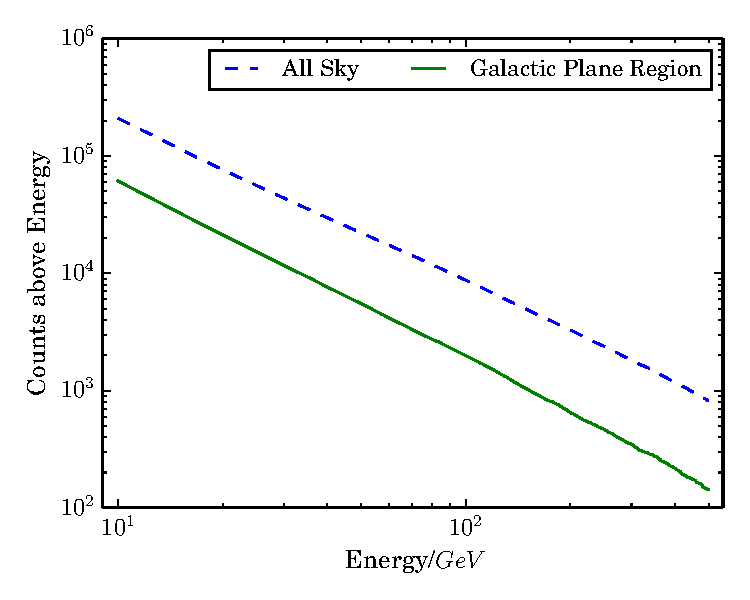
\includegraphics[width=0.5\textwidth]{figures/counts.pdf}
  \caption{Fermi/\textit{LAT} cosmic-ray events detected above energies to illustrate the energy distribution of cosmic-ray detections between 10 and 500 GeV.}
  \end{center}
\end{wrapfigure}

The 5-year LAT data is used within a specified energy band between 10 and 500 GeV, covering much of the region of relevance at the cross-over of GeV and TeV studies in a well-defined and understood manner. The cosmic-rays detected for this dataset above a given lower energy cut-off are illustrated in Figure 2, for which the steep fall-off in higher-energy detections typical of GeV and TeV studies is evident.

Table 1 quantifies the counts shown in the figure by outlining the counts seen in each of these regions at approximately logarithmically even energy binnings within the range of the selected events (and subsequent counts map).

\begin{table}
\centering
\begin{tabular}{|c|c|c|c|}
\hline
\multirow{2}{*}{\textbf{Energy, $E$/$GeV$}} & \multicolumn{2}{|c|}{\textbf{Number of LAT Events}}\\
 & All Sky & Galactic Plane \\\hline
$10 < E \leq 30$ & 165564 & 49417 \\\hline
$30 < E \leq 100$ & 34826 & 9643 \\\hline
$100 < E \leq 500$ & 7911 & 1838 \\\hline
$ E > 500$ & 818 & 143 \\\hline
\end{tabular}
\caption{Quantitative Illustration of Events observed between 10 GeV and 500 GeV}
\end{table}

\subsection{\textit{Fermi}/LAT PSF}


Studies have shown that the \textit{Fermi}/LAT PSF is largely spatially independent at energies above 10 GeV.


In the cases where PSF convolution is required for the 10 - 500 GeV energy band data study, the PSF is taken to be the that at the Galactic Center position, at an energy within the band determined by the method outlined by Lafferty \& Wyatt in %\cite{lw}
, assuming a powerlaw of spectral index -2.7... TODO: Check this.

. This is then assumed to be the true PSF for the data in this energy range, and assumed to be spatially independent (as variations are minor). PSF information is outlined Table 3.


\begin{wrapfigure}{l}{0.4\textwidth}
\centering
\resizebox{0.3\textwidth}{!}{
\begin{tabular}{|c|c|}
\hline
\textbf{Containment/$\%$} & \textbf{Radius/$deg$}\\\hline
68.0 & 0.150 \\\hline
95.0 & 0.867 \\\hline
\end{tabular}}
\caption{\textit{Fermi}/LAT PSF Containment}
\end{wrapfigure}


\section{Study Specifications}

\subsection{Analysis Regions}

The study specifically considers the ability of methods to differentiate between source and background emission. As such, it is sensible to choose regions of study restricted to the Galactic Plane as minimal diffuse or background emission is observed away from low galactic latitudes. As such, an analysis region of galactic latitude $-5 < b < 5$ and galactic longitude $-100 < l < 100$ is chosen to encompass the majority of the observed galactic emission, without deviating into the extra-galactic regime. This ensures regions of high source population density (at low latitudes and longitudes around the galactic center) as well as regions where background emission is likely to be more prevalent with fewer sources (away from the galactic plane and center) to allow methods to be tested in a range of situations: from regions of close, bright overlapping sources to areas sparesly populated by sources.

\section{Simulation}


The input images applied to the algorithm may take a number of forms. In the first instance, these may be observational data provided as a counts map and, indeed, the application of the process to true data is the ultimate aim of this work, so as to provide a true measure of background Milky Way emission above 10 GeV. This is however an endpoint. To evaluate and study the method itself, an input must be chosen for which a known source population and flux contribution is used in combination with a known background flux contribution. This may be done in either taking an observationally-derived high-energy catalog (for instance the fermi 1FHL catalog of point sources) and adding these point sources to a background model, or simulating realistic galactic source population catalogs to overlay onto such a background emission model. In both cases, realistic simulated images must be developed in order to reflect the nature of the datasets to which the algorithm itself will ultimately be applied. This means physically-motivated background maps (derived from gas column density measurements) should be used in conjunction with either survey catalogs of observed sources or simulated galactic populations with a strong base in physical reasoning.


In this study, both simulation methods are considered. The nature of the simulated and data inputs are summarized in Table (TODO).


\subsection{Observationally-inpired Simulation}
- TODO: 1FHL sources plus Fermi diffuse background model
- Describe, summarise parameters and proportion of diffuse and source flux.

\subsection{Model-inspired Simulation}

An alternative to the simulation method above is to substitute the observational catalog with a model-inspired galactic source catalog simulation. This, in turn, can be added to a diffuse background model in a similar manner to before.

While care is required in choosing suitable parameters to simulate a physically realistic galaxy source population, catalog simulation offers the advantage of greater sample of test galaxies - true source catalogs only exist for our own galaxy, offering a very limited test base.

A recent catalog study was undertaken as part of the work in the Fermi 1FHL catalog, and is documented in the accompanying paper \cite{1fhl}. This study considered a reference galaxy of a similar source population and distribution to the Milky Way, and two further simulations aiming to provide test cases for source detection with different proportions of bright and faint sources, allowing the influence of these different populations upon the source detection methods and resulting source catalog to be understood. 

In this work, we use galactic simulations for two reasons. The first is to increase the number of test cases upon which the source separation algorithm can be tests, while the second is to gain a better understanding of how the algorithm is able to differentiate between sources and diffuse emission under different conditions - for instance, with a larger unresolved population or a more dense source distribution. This falls very much in line with the studies undertaken in the 1FHL catalog galaxy simulations, and as such we replicate the quoted simulation parameters \cite[p.59]{1fhl} for this work. This is outlined below.

In line with \cite{Strong}, it is assumed that the luminosity function of the $\gamma$-ray source population between two limits $L_{\gamma, min}$ and $L_{\gamma, max}$ follows a simple power law of index -1.5, as per equation (1).

\begin{equation}
N(L_{\gamma}) = \frac{dN}{dL} = L_{\gamma}^{-1.5}
\end{equation}

Additionally, it is taken that the spatial distribution of pulsars offers representative example of spatial distribution of a galactic $\gamma$-ray source population \cite[p.2]{Strong}. Thus we use a galactocentric $(R, z)$ pulsar distribution model \cite[p.7]{Lorimer} to distribute sources, outlined in equation (2) - a gamma function - for the $\rho(R)$ radial source density distribution, and equation (3) - an exponential function - for the $\rho(z)$ distribution.

\begin{equation}
\rho(R) = A\left(\frac{R}{R_{\astrosun}}\right)^{B} \exp\left(-C\left[\frac{R-R_{\astrosun}}{R_{\astrosun}}\right]\right)
\end{equation}

\begin{equation}
\rho(z) = D \exp(-|z|/E)
\end{equation}

$R_{\astrosun}$ is taken as the radial position of the Sun with respect to the galactic center while $A, B, C, D$ and $E$ are model parameters discussed in the following. Standard Monte-Carlo methods are used to sample $\rho(L_{\gamma}, R, z)$ throughout the simulated galaxy and then the resulting distribution is normalized and scaled at $R_{\astrosun}$ to set an appropriate value to $A = \rho_{\astrosun}$ as the population density of the sun. Since the true radial distribution is the product $\rho(R, z) = \rho(R) \times \rho(z)$ and the overall normalization of $\rho(R, z)$ is set in $\rho(R)$ by the parameter $A$, the second $\rho(z)$ normalization parameter $D$ may be set to 1.

In line with the 1FHL study, the radial distribution peaks at 4 kpc - thus $B = 4$ and $C = R_{\astrosun}$ to fall in line with this. The $\rho(z)$ exponential scale is set to 0.5 kpc (so $E=0.5$).  These are summarised in Table 3. 

\begin{wrapfigure}{l}{0.4\textwidth}
\centering
\resizebox{0.3\textwidth}{!}{
\begin{tabular}{|c|c|}
\hline
\textbf{Model Parameter} & \textbf{Value}\\\hline
$A$ & $\rho_{\astrosun}$ kpc$^{-2}$ \\\hline
$B$ & 4 \\\hline
$C$ & $R_{\astrosun}$ kpc \\\hline
$D$ & 1 kpc$^{-1}$\\\hline
$E$ & 0.5 kpc \\\hline
\end{tabular}}
\caption{Galaxy Modelling Parameter Values.}
\end{wrapfigure}

A reference model is defined with $\rho_{\astrosun} = 3 \text{kpc}^{-3}$ with a minimum $\gamma$ luminosity $L_{\gamma, min} = 10^{34} \text{ph s}^{-1}$ and maximum $\gamma$ luminosity $L_{\gamma, min} = 10^{37} \text{ph s}^{-1}$. Two comparison models - both of higher population densities at the position of the sun, and lower luminosity bounds - are also considered. The relevant parameters of these three models are outlined in Table 3.

\begin{table}
\centering
\resizebox{\textwidth}{!}{
\begin{tabular}{|c|c|c|c|}
\hline
\textbf{Source Model} & \textbf{Population Density at the Sun/$kpc^{-3}$} & \textbf{Minimum Luminosity/$ph s^{-1}$} & \textbf{Maximum Luminosity/$ph s^{-1}$}\\\hline
Reference Simulation & 3 & $10^{34}$ & $10^{37}$\\\hline
Simulation 1 & 10 & $4 \times 10^{33}$ & $4 \times 10^{36}$ \\\hline
Simulation 2 & 30 & $1.5 \times 10^{33}$ & $1.5 \times 10^{36}$ \\\hline
\end{tabular}}
\caption{Parameters for 10 - 500 GeV Galaxy Population Simulations.}
\end{table}

- If space is left, include LogN/LogS distribtions of these simulated galaxies, and the 1FHL model.

\subsection{Flux Distrubtions}

The proportion of the total flux of the models in the galactic plane may be considered as an intitial measure of the galactic plane source density in the three simulated cases. Table 4 compares each of the simulated catalogs against the 1FHL catalog to offer a comparison, and to provide an indication of the distribution and density of each source population. It should be noted that the considerably lower relative galactic flux contribution of the 1FHL catalog-based model compared to the purely simulated models is likely to be due to experimentally unresolved sources in the galactic plane which are not detected by the LAT and so do not appear within the source catalog. A bias exists due to the background galactic emission, meaning that point sources away from the galactic plane may be more readily resolved and thus are more likely to appear in the catalog detections. A discussion can be found in chapter 6 of the 1FHL catalog paper \cite[p.59]{1fhl} for these models, and it is shown that in the case of the reference model, the $log(N)/log(S)$ source flux distribution plot matches the 1FHL catalog above the effective experimental detection threshold.

\begin{table}
\centering
\resizebox{\textwidth}{!}{
\begin{tabular}{|c|c|c|c|}
\hline
\textbf{Source Model} & \textbf{Total Flux/ph cm$^{-2}$ s$^{-1}$} & \textbf{Flux in Galactic Region/ph cm$^{-2}$ s$^{-1}$} & \textbf{Proportion of Flux in Galactic Region/\%}\\\hline
\testit{Fermi} 1FHL Catalog > 10 GeV & $1.60\text{e}^{-7}$ & $2.84\text{e}^{-9}$ & 1.77\\\hline
Reference Simulation & $9.96\text{e}^{-8}$ & $1.70\text{e}^{-8}$ & 17.1\\\hline
Simulation 1 & $1.93\text{e}^{-7}$ & $1.94\text{e}^{-8}$ & 10.0 \\\hline
Simulation 2 & $1.93\text{e}^{-7}$ & $1.99\text{e}^{-8}$ & 10.3 \\\hline
\end{tabular}}
\caption{Galactic plane fluxes for source population catalogs.}
\end{table}

Before application to the source separation algorithm, the 1FHL and simulated catalogs are added to the integrated Fermi Diffuse background model \verb|gll_iem_v05_rev1.fit| between 10 GeV and 500 GeV to produce source/diffuse test cases. The integral flux of the background model in the galactic plane region contributes an all-sky flux of $4.21\text{e}^{-6} \text{ph cm}^{-2}\text{s}^{-1}$, of which $2.85\text{e}^{-7} \text{ph cm}^{-2}\text{s}^{-1}$ ($6.77\%$) is contributed by the galactic plane region.


\section{Results}

The results of this study may be categorized as those relating the the simulated inputs used to understand the algorithm, and those relating to the applicaiton of the separation algorithm to real Fermi-LAT data.

\subsection{Simulation Results}

\begin{wrapfigure}{l}{0.6\textwidth}
\centering
\resizebox{0.6\textwidth}{!}{
\begin{tabular}{|c|c|c|}
\hline
\textbf{Source Model} & \textbf{True Source} & \textbf{Recovered Source}\\
\textbf{(\& Fermi Diffuse Background)} & \textbf{Flux Fraction/\%} & \textbf{Flux Fraction/\%}\\\hline
Fermi 1FHL Catalog > 10 GeV & 0.987 & \\\hline
Reference Simulation & 5.63 & \\\hline
Simulation 1 & 6.37 & \\\hline
Simulation 2 & 6.52 & \\\hline
\end{tabular}}
\caption{Galaxy Modelling Parameter Values.}
\end{wrapfigure}

\begin{wrapfigure}{c}{\textwidth}
  \begin{center}
      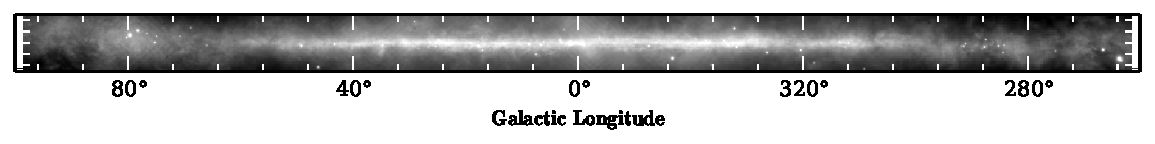
\includegraphics[width=\textwidth]{figures/1FHL.pdf}
  \caption{1FHL Catalog input image.}
  \end{center}
\end{wrapfigure}

\begin{wrapfigure}{c}{\textwidth}
  \begin{center}
      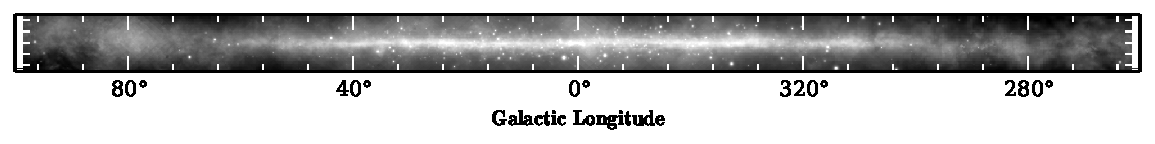
\includegraphics[width=\textwidth]{figures/SIM1.pdf}
  \caption{Reference Simulation galaxy input image.}
  \end{center}
\end{wrapfigure}

\begin{wrapfigure}{c}{\textwidth}
  \begin{center}
      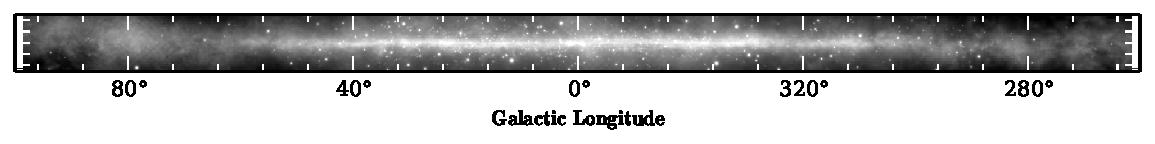
\includegraphics[width=\textwidth]{figures/SIM2.pdf}
  \caption{Galaxy simulation 1 input image.}
  \end{center}
\end{wrapfigure}

\begin{wrapfigure}{c}{\textwidth}
  \begin{center}
      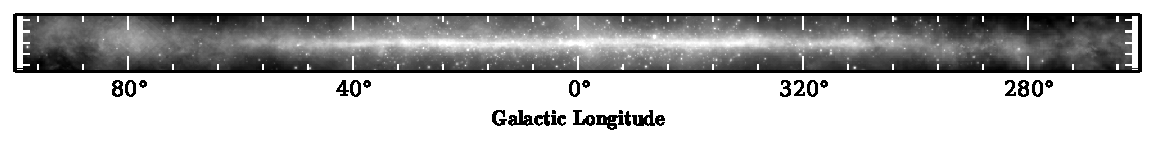
\includegraphics[width=\textwidth]{figures/SIM3.pdf}
  \caption{Galaxy simulation 2 input image.}
  \end{center}
\end{wrapfigure}
\\
- A few images, but mainly results should be summarized in a table here.



results for
- 1FHL + fermi diffuse\\
- Simulated galaxy 1 + fermi diffuse\\
- Simulated galaxy 2 + fermi diffuse\\
- Simulated galaxy 3 + fermi diffuse\\

- Should include:\\
    - Original background counts\\
    - recovered background counts\\
    - original source counts\\
    - recovered source counts\\
    - original number of sources\\
    - recovered number of sources\\
    - latitude and longitude profile of background before and after\\
    - latitude and longitude profile of sources before and after
        (these will give an idea as to how good the method in question was at separating sources in sparse and dense regions)

\subsubsection{Fermi-LAT Data Results}

TODO

\section{Conclusions}


\section{Summary}
These methods are included in the affiliated astropy open-source package, gammapy \cite{Deil}.

\begin{thebibliography}{99}

\bibliographystyle{plain}
\bibliography{references}


\end{thebibliography}
\end{document}


